% s1: the problem, as it is posed. ASCII only.
\section{Introduction: the problem and the proposal}

\subsection*{What I mean by Helike}

Before I follow Helike through this theory, I want to say what she is. Helike is the name I give to an explicitly
identified family of deformation modes of a Yang--Mills field on a Berger sphere: a three-sphere stretched along a
preferred family of circles. A mode tells me how the field changes, point by point. It is a pattern of field
variation, not a new particle placed inside the theory.

The Yang--Mills Hessian measures the quadratic energy variation about a background field. Its eigenvalue gives
a number; its eigenvector gives the pattern that number belongs to. My starting point is to follow that pattern,
not only its number. My earlier work identifies Helike exactly and establishes the domain in which she occupies
the bottom of that Hessian spectrum~\cite{ByEnough,Floor}. Here I ask what quantum dynamics makes of this geometric
mode: how it contributes to an excitation, competes with another shape, and responds to the finer modes and the
size of the space. A Hessian mode and a full quantum state are different objects; following the connection is part
of this theory.

In her simplest homogeneous form, Helike is a \emph{doublet}: two real patterns spanning one two-dimensional mode
space (Figure~\ref{fig:helike-doublet}). Their coefficients are constant in the moving frame; the frame itself varies
over the sphere. At a circle-symmetric background the two partners have the same Hessian eigenvalue.

\par\Needspace{7\baselineskip}
\emph{Charge 2} describes their rotation law, not electric charge. Rotate the spatial frame and the compensating
colour frame together through an angle $\theta$: the pair of coefficients turns through $2\theta$. A $45^\circ$
rotation takes the first pattern to the second; a $90^\circ$ rotation gives the negative of the first, not the same
pattern. A $180^\circ$ rotation returns it. This is the precise sense of the turn shown here, not a drawing of a
material ribbon or a trajectory through space.

\begin{figure}[!htbp]
\centering
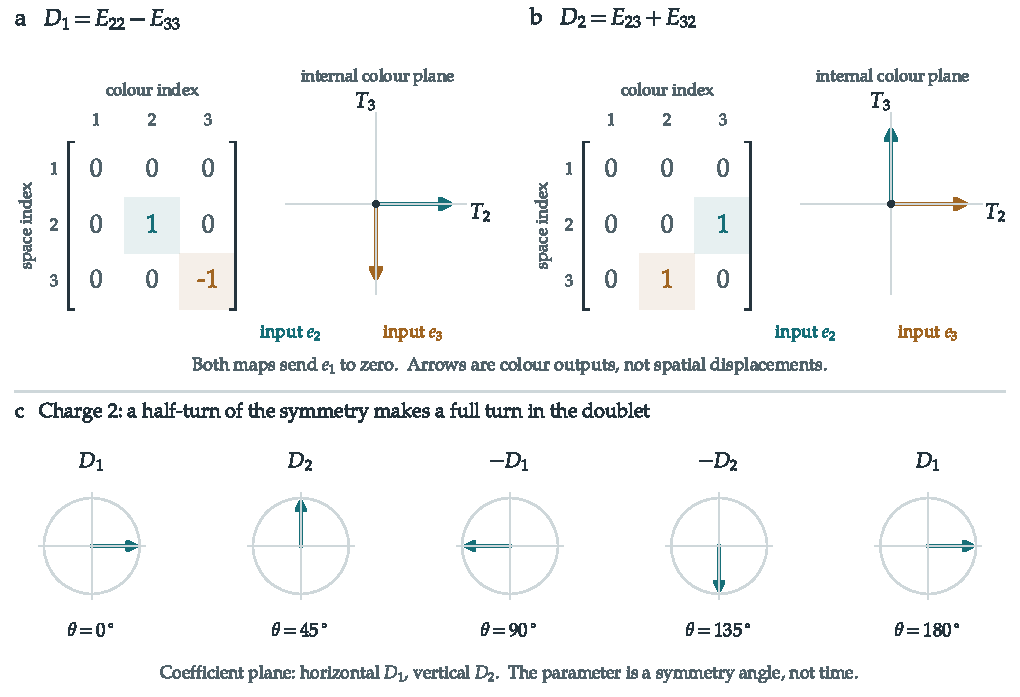
\includegraphics[width=\linewidth]{figures/helike-doublet.pdf}
\caption{\textbf{Helike's actual homogeneous doublet in the convention of \S4.}
$D_1=E_{22}-E_{33}$ and $D_2=E_{23}+E_{32}$, with $E_{ka}$ equal to one in row $k$, column $a$, and zero elsewhere.
Rows are spatial inputs $e_k$; columns are internal colour components $T_a$.
The arrows show $b_D(e_k)=\sum_a D_{ka}T_a$: teal for input $e_2$, gold for input $e_3$.
They lie in the colour plane, not the spatial tangent plane. Both maps annihilate $e_1$.
Below, $R_\theta$ rotates $e_2$ toward $e_3$ (and $T_2$ toward $T_3$), giving
$R_\theta D_1R_\theta^T=\cos(2\theta)D_1+\sin(2\theta)D_2$.
The two complex combinations have charges $\pm2$; the plot uses the real pair.
The matrices are unnormalized, each with Frobenius norm $\sqrt2$; divide by $\sqrt2$ for unit matrix norm.
This shows the homogeneous member, not the higher-harmonic family or a global $L^2$ normalization.}
\label{fig:helike-doublet}
\end{figure}

\clearpage
\subsection*{The proposed mechanism}

\textbf{The theory.} Topology organizes the field's possible routes; geometry and kinetic energy give them their costs;
quantum dynamics determines the lowest excitation. I propose that the mass gap is the lowest note of this combined
structure, carried by a shape that leans toward a winding-changing route. The fine grain dresses that shape, and the
note is inherited all the way out to infinite space. If the theory is true, it says five things.
\begin{enumerate}
\item \textbf{The gap has a name:} in a small room it is carried by Helike, a twisting shape of charge~2 under the room's rotation symmetry, or by
her competitor, a breathing shape of charge~0, and as the room grows the carrier changes only at exact, countable
switches (\S4--5). \item \textbf{The landscape gives the carriers their costs:} the reduced potential is the squared slope
of Chern--Simons, measured with the field-space metric. The competitor follows the one downhill direction of
Chern--Simons at the winding-one vacuum: the field's first step toward the other winding vacuum. The quantum ordering
comes from the potential and kinetic energy together. This suggests a mechanism for the scalar glueball being
lightest (\S5). \item \textbf{Tensor-like and scalar-like channels trade places at a
calculable point,} $s_0^*(t)=(t+2)(\sqrt{t+8}-\sqrt t)/(4\sqrt t)$, which is $1.1436$ at $t=3$ at harmonic order; the switches registered at stronger coupling rise from it (\S5). \item \textbf{The
fine grain cannot erase the note:} the computed logarithmic divergence has the asymptotically free coefficient
$b_0=22/3$; finite and kinetic dressing must still be controlled (\S6). \item \textbf{The infinite world is the last room:} infinite
space is the end of a family of spheres, and the gap in units of the theory's scale stays uniformly above zero,
including at that end (\S7--8).

\end{enumerate}
Simulations provide evidence for a gap and scalar glueball ordering; perturbation theory establishes asymptotic freedom,
not the nonperturbative gap. My proposal is to connect those observations through one geometric mechanism.


The central conjecture is stated after the geometric definitions in \S2. I retain the standing of each supporting
statement beside it; Appendix~\ref{app:register} collects the complete status and coverage maps.

\subsection*{The problem, as it is posed}

The target is not mine. It is the Millennium Prize problem as Jaffe and Witten wrote it~\cite{JaffeWitten}. For every
compact simple gauge group $G$ (the symmetry group of the field, such as $SU(2)$ or $SU(3)$), construct quantum
Yang--Mills theory on four-dimensional space-time $\mathbb R^4$ and show two things. First, it exists as a genuine
quantum field theory: it satisfies axioms at least as strong as Wightman's~\cite{StreaterWightman}, or in Euclidean form
those of Osterwalder and Schrader~\cite{OS73,OS75} (Euclidean invariance, reflection positivity, regularity, clustering),
from which a relativistic theory is reconstructed; it has local field operators for the gauge-invariant polynomials in
the curvature $F$, such as $\mathrm{tr}\,F^2$; at short distance it agrees with perturbation theory and asymptotic
freedom~\cite{GrossWilczek73,Politzer73}; and it is non-trivial, not a free field in disguise. Second, it has a mass gap:
the spectrum above the vacuum begins at a strictly positive, finite energy. Normalized states
orthogonal to the vacuum have energy expectation at least $\Delta>0$; a superposition with a vacuum component need not.

The problem is hard because of two infinities. The \emph{ultraviolet} is the fine grain: zoom in and the field has ever
finer ripples, infinitely many, which must be controlled together (renormalization). The \emph{infrared} is the growing
room: zoom out, and the gap must survive in infinite space, exactly where the coupling becomes strong and no small
parameter is left. Every computation, mine included, cuts off one or both, with a lattice of spacing $a$ or a room of
finite size. The difficulty is to remove the scaffolding and keep the answer.

\begin{claim}{OPEN}{The Clay target}\label{b:clay}
For $G=SU(2)$, and then every compact simple $G$, quantum Yang--Mills theory on $\mathbb R^4$ exists with every
property above (OS and so Wightman axioms, local fields, short-distance agreement, non-triviality, a unique vacuum), and
its Hamiltonian has nothing in $(0,\Delta)$, with a nonempty excitation spectrum and finite first spectral threshold
$m\ge\Delta=c\,\Lambda>0$. Here $\Lambda$ is an energy scale in a fixed renormalization scheme,
and $c>0$ a dimensionless number. I work at vacuum angle $\theta=0$.
\evidence{The problem itself~\cite{JaffeWitten}. My register splits it into 29 lines and maps every clause to them
(Table~\ref{tab:clay}); it rests on four hypotheses, H3, H4$'$, H6, H7~\cite{ClosedSet}.}
\lines{1--29}
\end{claim}

\subsection*{Relation to earlier work}

What has been done shows where the wall is. Interacting theories were built in two and three
dimensions~\cite{GlimmJaffe}; two-dimensional Yang--Mills is solved exactly~\cite{Migdal75,GrossWitten80,Sengupta97,Levy03};
on a lattice at strong coupling the gap is a theorem~\cite{OsterwalderSeiler78,ShenZhuZhu23}, at the wrong end of the
coupling. In four dimensions Ba{\l}aban
controlled the ultraviolet in a finite box~\cite{Balaban}, and Magnen, Rivasseau and S\'en\'eor built the $SU(2)$
Schwinger functions with an infrared cutoff kept~\cite{MRS93}. Nobody has removed the infrared cutoff. Physically the
gap is not in doubt: simulations find a lightest glueball, a scalar $0^{++}$~\cite{MorningstarPeardon99}.

Simulations show a gap with the scalar lightest~\cite{MorningstarPeardon99};
perturbation theory shows asymptotic freedom~\cite{GrossWilczek73,Politzer73}; strong-coupling expansions prove a gap at
the strong-coupling end~\cite{OsterwalderSeiler78}. My theory proposes a geometric connection between them:
topology organizes the landscape's routes; its geometry makes the downhill Chern--Simons direction locally soft;
quantum dynamics combines that landscape with kinetic energy, and the fine grain dresses the resulting carrier.
In this picture they are parts of one mechanism: the
lowest note of the folded space of field shapes, named in the small room and followed to infinite space. The finite-volume road
is L\"uscher's and van Baal's~\cite{Luscher83,KollerVanBaal88,vanBaal00}; the stretched sphere, the identified floor, the
named carrier, the sources, the harmonic switch and the proposed inheritance along scale are the route developed here.

The scale $\Lambda$ is where the problem turns geometric. The classical equations contain no length; the quantum theory
makes an energy scale through the running coupling; in units $\hbar=c=1$, $1/\Lambda$ is the associated length.
A gap that is a pure number times that energy scale is a
property of shape, not of any box. So I begin with the shape.
